The application server provides the required execution environment for business
services to be deployed and executed within. The application server is responsible
for realizing the business layer.

\subsection{Architecture Requirements}
The architectural requirements include refined quality requirements and architecural
responsibilities. The applicatoin server however doesn't include additional
architecture constraints other than those specified in section \ref{sec:systemArchitecturalConstraints}

\subsubsection{Access and Integration Requirements}
The stated access and integration requirements in section \ref{sec:accessIntegrationRequirementsManagementSystem}
need to be propegated down to this lower level component. The application server
will be mainly responsible for exposing these channels realized by other lower
level components.

Further more stated quality requirements in section \ref{sec:qualityRequirementManagementSystem}
need to also be propegated down to this layer as much of the quality
requirements will realized by the application server. Further refinement of the
quality requirements is however provided.

\subsubsection{Quality Requirements}
\paragraph{Flexibility}
The application server should allow for the flexable deployment of any layer at
any-time with the minimal system downtime and no lose of information to occur
because the system is down. This is especially important as one doesn't want to
lose the results of users, should they be communicated back to the system
during a time which it is down.

\paragraph{Security}
The application should allow for both the authentication and autherization of
users. It is important to note the difference between these similar words.

Authentication is a systematic process of proof to determine whether a said
party is genuine.  Authorization is the verification of whether the said party
has the required privilidges to perform the requested action on or in a resource.

The application server should support authentication within some neutral framework
to allow for future expansion of authentication methods such as LDAP and in addition
should support authorization throught a role-based system. Users access to the
system should happen soley through the approved access channels as to prevent users
from directly accessing the datbase, message bus and other components directly.


\subsubsection{Architectural Responsibilities}
The architectural responsibilities of the persistence API are shown in
Figure \ref{fig:applicationServerResponsibilities}
\begin{figure}[H]
	\begin{center}
	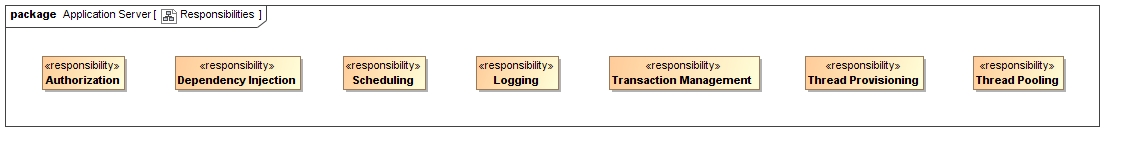
\includegraphics[scale=0.4]{../Diagrams and Charts/Application Server/Responsibilities.jpg}
	\caption{The architectural responsibilities of the Application Server}
	\label{fig:applicationServerResponsibilities}
	\end{center}
\end{figure}

\subsubsection{Architecture Constraints}
\subsection{Architecture Design}
\subsubsection{Tactics}
\subsubsection{Architectural Components}
The architectural components of the Application Server are shown in Figure \ref{fig:applicationServerResponsibilityAllocation}
\begin{figure}[H]
	\begin{center}
	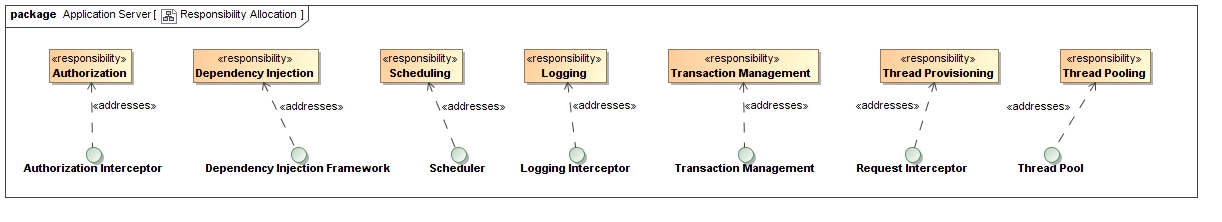
\includegraphics[scale=0.4]{../Diagrams and Charts/Application Server/ResponsibilityAllocation.jpg}
	\caption{The abstract components to which the architectural responsibilities are assigned.}
	\label{fig:applicationServerResponsibilityAllocation}
	\end{center}
\end{figure}

\subsubsection{Frameworks and Technologies}
\paragraph{Concrete Realization of Architectural Components}
The components realizing the architectural responsibilities specified in figure \ref{fig:applicationServerResponsibilities} are shown in figure \ref{fig:applicationServerResponsibilityRealization}.
\begin{figure}[H]
	\begin{center}
	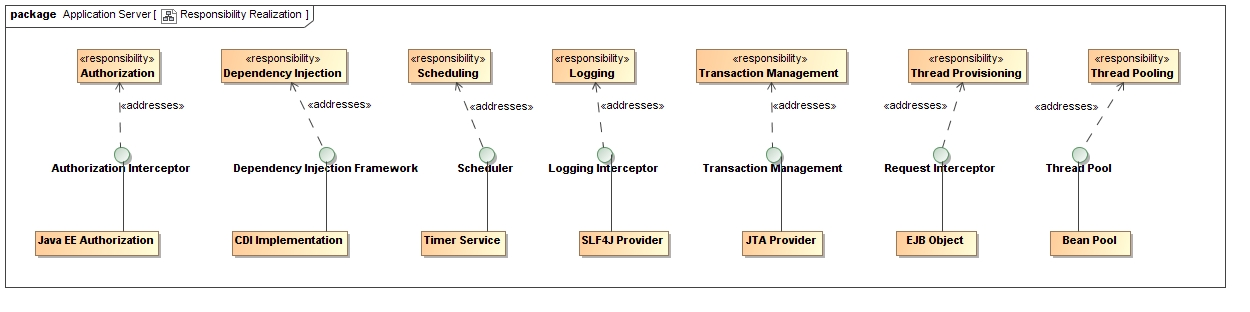
\includegraphics[scale=0.4]{../Diagrams and Charts/Application Server/ResponsibilityRealization.jpg}
	\caption{The components in Java-EE addressing the architectural responsibilities of the application server}
	\label{fig:applicationServerResponsibilityRealization}
	\end{center}
\end{figure}

\paragraph{Concepts and Constraints for Application Components}
The programming methodology used which will be used to code the business services is know as Design by Contract (DbC). With the DbC paradigm, a \textit{service contract} represents the requirements for a service, including pre- and post-conditions. All pre-conditions need to be fulfilled before the service in questions will render any services. A \textit{service} within the DbC methodology refers to a concrete implementation of a service contract. 

Furthermore services should be stateless, i.e. no state is maintained across service requests, but rather state is preserved in domain objects which themselves should contain no business logic code. These domain objects are usually persisted to a persistence provider for later retrieval.

Within the Java-EE architecture the DbC is executed as follow
\begin{itemize}
	\item Service contracts are mapped onto Java Interfaces
	\item Services are classes that implement the required interface as a stateless session bean
	\item Domain objects are mapped onto Plain Old Java Objects (POJO)'s
\end{itemize}